%==================================================================================
%=============================================================================

\section{Interfaces del subsistema: Gestión de proyectos}

\subsection{CU03 Crear Proyecto}
{
\justify
\color{blue}{\textbf{Objetivo}}
}

%------------------------------------------------------------------
\justify
En esta pantalla permite al Lider de proyecto crear un proyecto.
%------------------------------------------------------------------
{
\justify
\color{blue}{\textbf{Diseño}}
}
%-------------------------------------------------------------------------------
\justify
En la figura \ref{fig:IU03} se muestra la pantalla, en donde el Lider de proyecto introducira los parametros necesarios para registrar un proyecto.

\begin{figure}[htb]
\centering
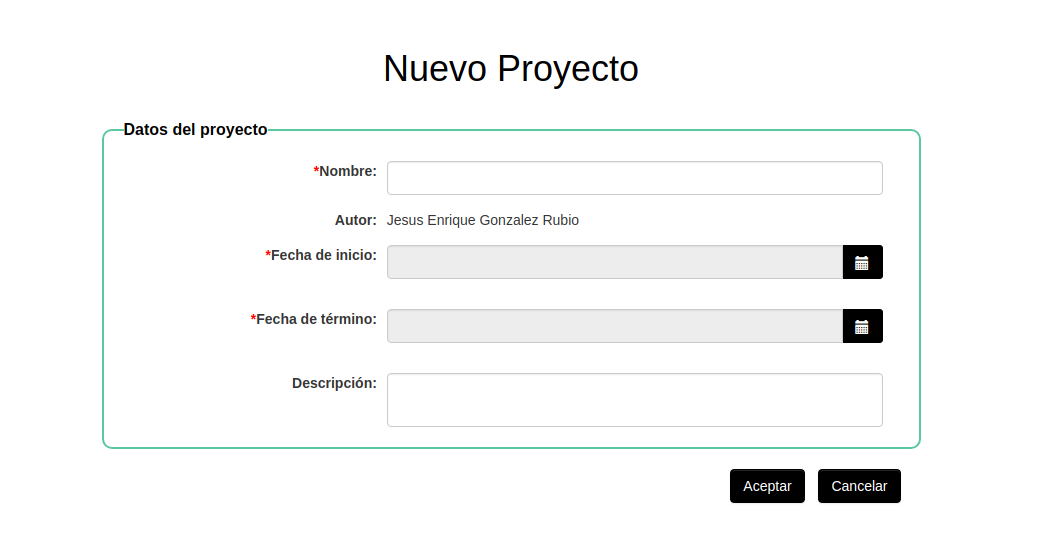
\includegraphics[width=0.8\textwidth]{./images/cu03-crear-proyecto.png}
\caption{Crear proyecto.} \label{fig:IU03}
\end{figure}